\subsection{Неоднородные системы. Теорема об общем решении неоднородной системы}

\begin{definition}
Система линейных алгебраических уравнений (СЛАУ) вида $AX = B$ называется \textbf{неоднородной}, если столбец свободных членов $B \neq \mathbf{0}$. Каждой такой системе можно поставить в соответствие \textbf{однородную систему} $AX = \mathbf{0}$ с той же основной матрицей $A$.
\end{definition}

Согласно теореме Кронекера--Капелли, неоднородная система совместна тогда и только тогда, когда ранг основной матрицы равен рангу расширенной матрицы ($\mathrm{rk}(A) = \mathrm{rk}(\tilde{A}) = R$).

\begin{theorem}[Об общем решении неоднородной системы]
Пусть дана совместная система $AX = B$. Если ранг матрицы $R$ меньше числа неизвестных $n$, то общее решение неоднородной системы $X_H$ представляется в виде:
\[ X_H = X_O + X_C \]
где $X_O$ — общее решение соответствующей однородной системы, а $X_C$ — некоторое частное решение неоднородной системы. 
Более развернуто (используя ФСР):
\[ X_H = c_1 Y_1 + c_2 Y_2 + \dots + c_{n-R} Y_{n-R} + X_C \]
где $\{Y_1, \dots, Y_{n-R}\}$ — фундаментальная система решений (ФСР) однородной системы $AX = \mathbf{0}$.
\end{theorem}

\begin{tcolorbox}[title=Доказательство, breakable]
Доказательство состоит из двух частей: проверки того, что сумма является решением, и того, что любое решение системы представляется в таком виде.

\textbf{1. Проверка решения (достаточность).}
Пусть $X_O$ — решение однородной системы ($AX_O = \mathbf{0}$), а $X_C$ — частное решение неоднородной системы ($AX_C = B$). Подставим их сумму в исходное уравнение, пользуясь дистрибутивностью умножения матриц:
\[ A(X_O + X_C) = AX_O + AX_C = \mathbf{0} + B = B \]
Следовательно, вектор $X_H = X_O + X_C$ является решением неоднородной системы.

\textbf{2. Полнота (необходимость).}
Покажем, что всякое решение системы можно получить по этой формуле. Пусть $X^*$ — произвольное решение неоднородной системы ($AX^* = B$). Рассмотрим вектор $Y = X^* - X_C$. Применим к нему матрицу $A$:
\[ AY = A(X^* - X_C) = AX^* - AX_C = B - B = \mathbf{0} \]
Это означает, что вектор $Y$ является решением однородной системы $AX = \mathbf{0}$. Следовательно, по теореме о структуре общего решения однородной системы, он может быть представлен как $X_O$ (линейная комбинация векторов ФСР):
\[ Y = c_1 Y_1 + \dots + c_{n-R} Y_{n-R} = X_O \]
Тогда исходное решение $X^*$ можно записать как:
\[ X^* = Y + X_C = X_O + X_C \]
Теорема доказана.
\end{tcolorbox}

\textbf{Геометрический смысл:}
Множество решений неоднородной системы представляет собой «плоскость» в пространстве $\R^n$, полученную путем параллельного переноса подпространства решений однородной системы на вектор частного решения $X_C$.
%\begin{figure}[h]
%    \centering
%    %\includegraphics... описание: чертеж с осями координат, где изображено подпространство U (решения однородной системы), проходящее через начало координат, и параллельная ему плоскость, смещенная на вектор x0 (частное решение).
%\end{figure}

\begin{figure}[h]
    \centering
    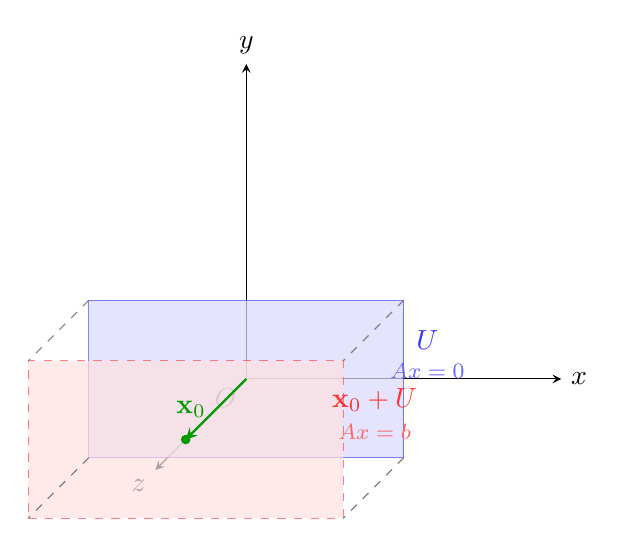
\begin{tikzpicture}[scale=1.0, >=stealth]

        % --- Оси координат ---
        \draw[->] (0,0,0) -- (4,0,0) node[right] {$x$};
        \draw[->] (0,0,0) -- (0,4,0) node[above] {$y$};
        \draw[->] (0,0,0) -- (0,0,3) node[below left] {$z$};
        \node[below left] at (0,0,0) {$O$};

        % --- Подпространство U (плоскость через начало координат) ---
        \filldraw[draw=blue!70, fill=blue!15, opacity=0.7]
            (-2,-1,0) -- (2,-1,0) -- (2,1,0) -- (-2,1,0) -- cycle;
        \node[blue!80] at (2.3, 0.5, 0) {$U$};
        \node[blue!60, font=\footnotesize] at (2.3, 0.1, 0) {$Ax=0$};

        % --- Смежный класс x0 + U (параллельная плоскость) ---
        \filldraw[draw=red!70, fill=red!12, opacity=0.7, dashed]
            (-2,-1,2) -- (2,-1,2) -- (2,1,2) -- (-2,1,2) -- cycle;
        \node[red!80] at (2.4, 0.5, 2) {$\mathbf{x}_0 + U$};
        \node[red!60, font=\footnotesize] at (2.4, 0.1, 2) {$Ax=b$};

        % --- Вектор x0 (частное решение) ---
        \draw[->, thick, green!60!black]
            (0,0,0) -- (0,0,2)
            node[midway, left] {$\mathbf{x}_0$};

        % --- Пунктирные линии, показывающие параллельность ---
        \draw[gray, dashed, thin] (-2,-1,0) -- (-2,-1,2);
        \draw[gray, dashed, thin] ( 2,-1,0) -- ( 2,-1,2);
        \draw[gray, dashed, thin] ( 2, 1,0) -- ( 2, 1,2);
        \draw[gray, dashed, thin] (-2, 1,0) -- (-2, 1,2);

        % --- Точка x0 на смежном классе ---
        \filldraw[green!60!black] (0,0,2) circle (1.5pt);

    \end{tikzpicture}
    \caption{Подпространство $U$ (решения $A\mathbf{x}=\mathbf{0}$) и смежный класс
    $\mathbf{x}_0 + U$ (решения $A\mathbf{x}=\mathbf{b}$), параллельный ему и
    смещённый на частное решение $\mathbf{x}_0$.}
    \label{fig:subspace-coset}
\end{figure}

\begin{tcolorbox}[title=Источники, colback=gray!10]
\begin{itemize}
  \item Лекция №\,4, тема «Неоднородные системы», временной отрезок 00:00--10:00
  \item PDF «Линейная алгебра\_compressed (1).pdf», раздел 5 «Неоднородные СЛАУ», стр. 15--16 (701--702)
  \item PDF «Марков Лекции по алгебре.pdf», Лекция 10, раздел 3, стр. 43--46 (798, 903--909)
  \item PDF «Вопросы», вопрос №\,9
\end{itemize}
\end{tcolorbox}
